\documentclass[main.tex]{subfiles}

\begin{document}

\begin{multicols}{2}


\begin{figure}[H]
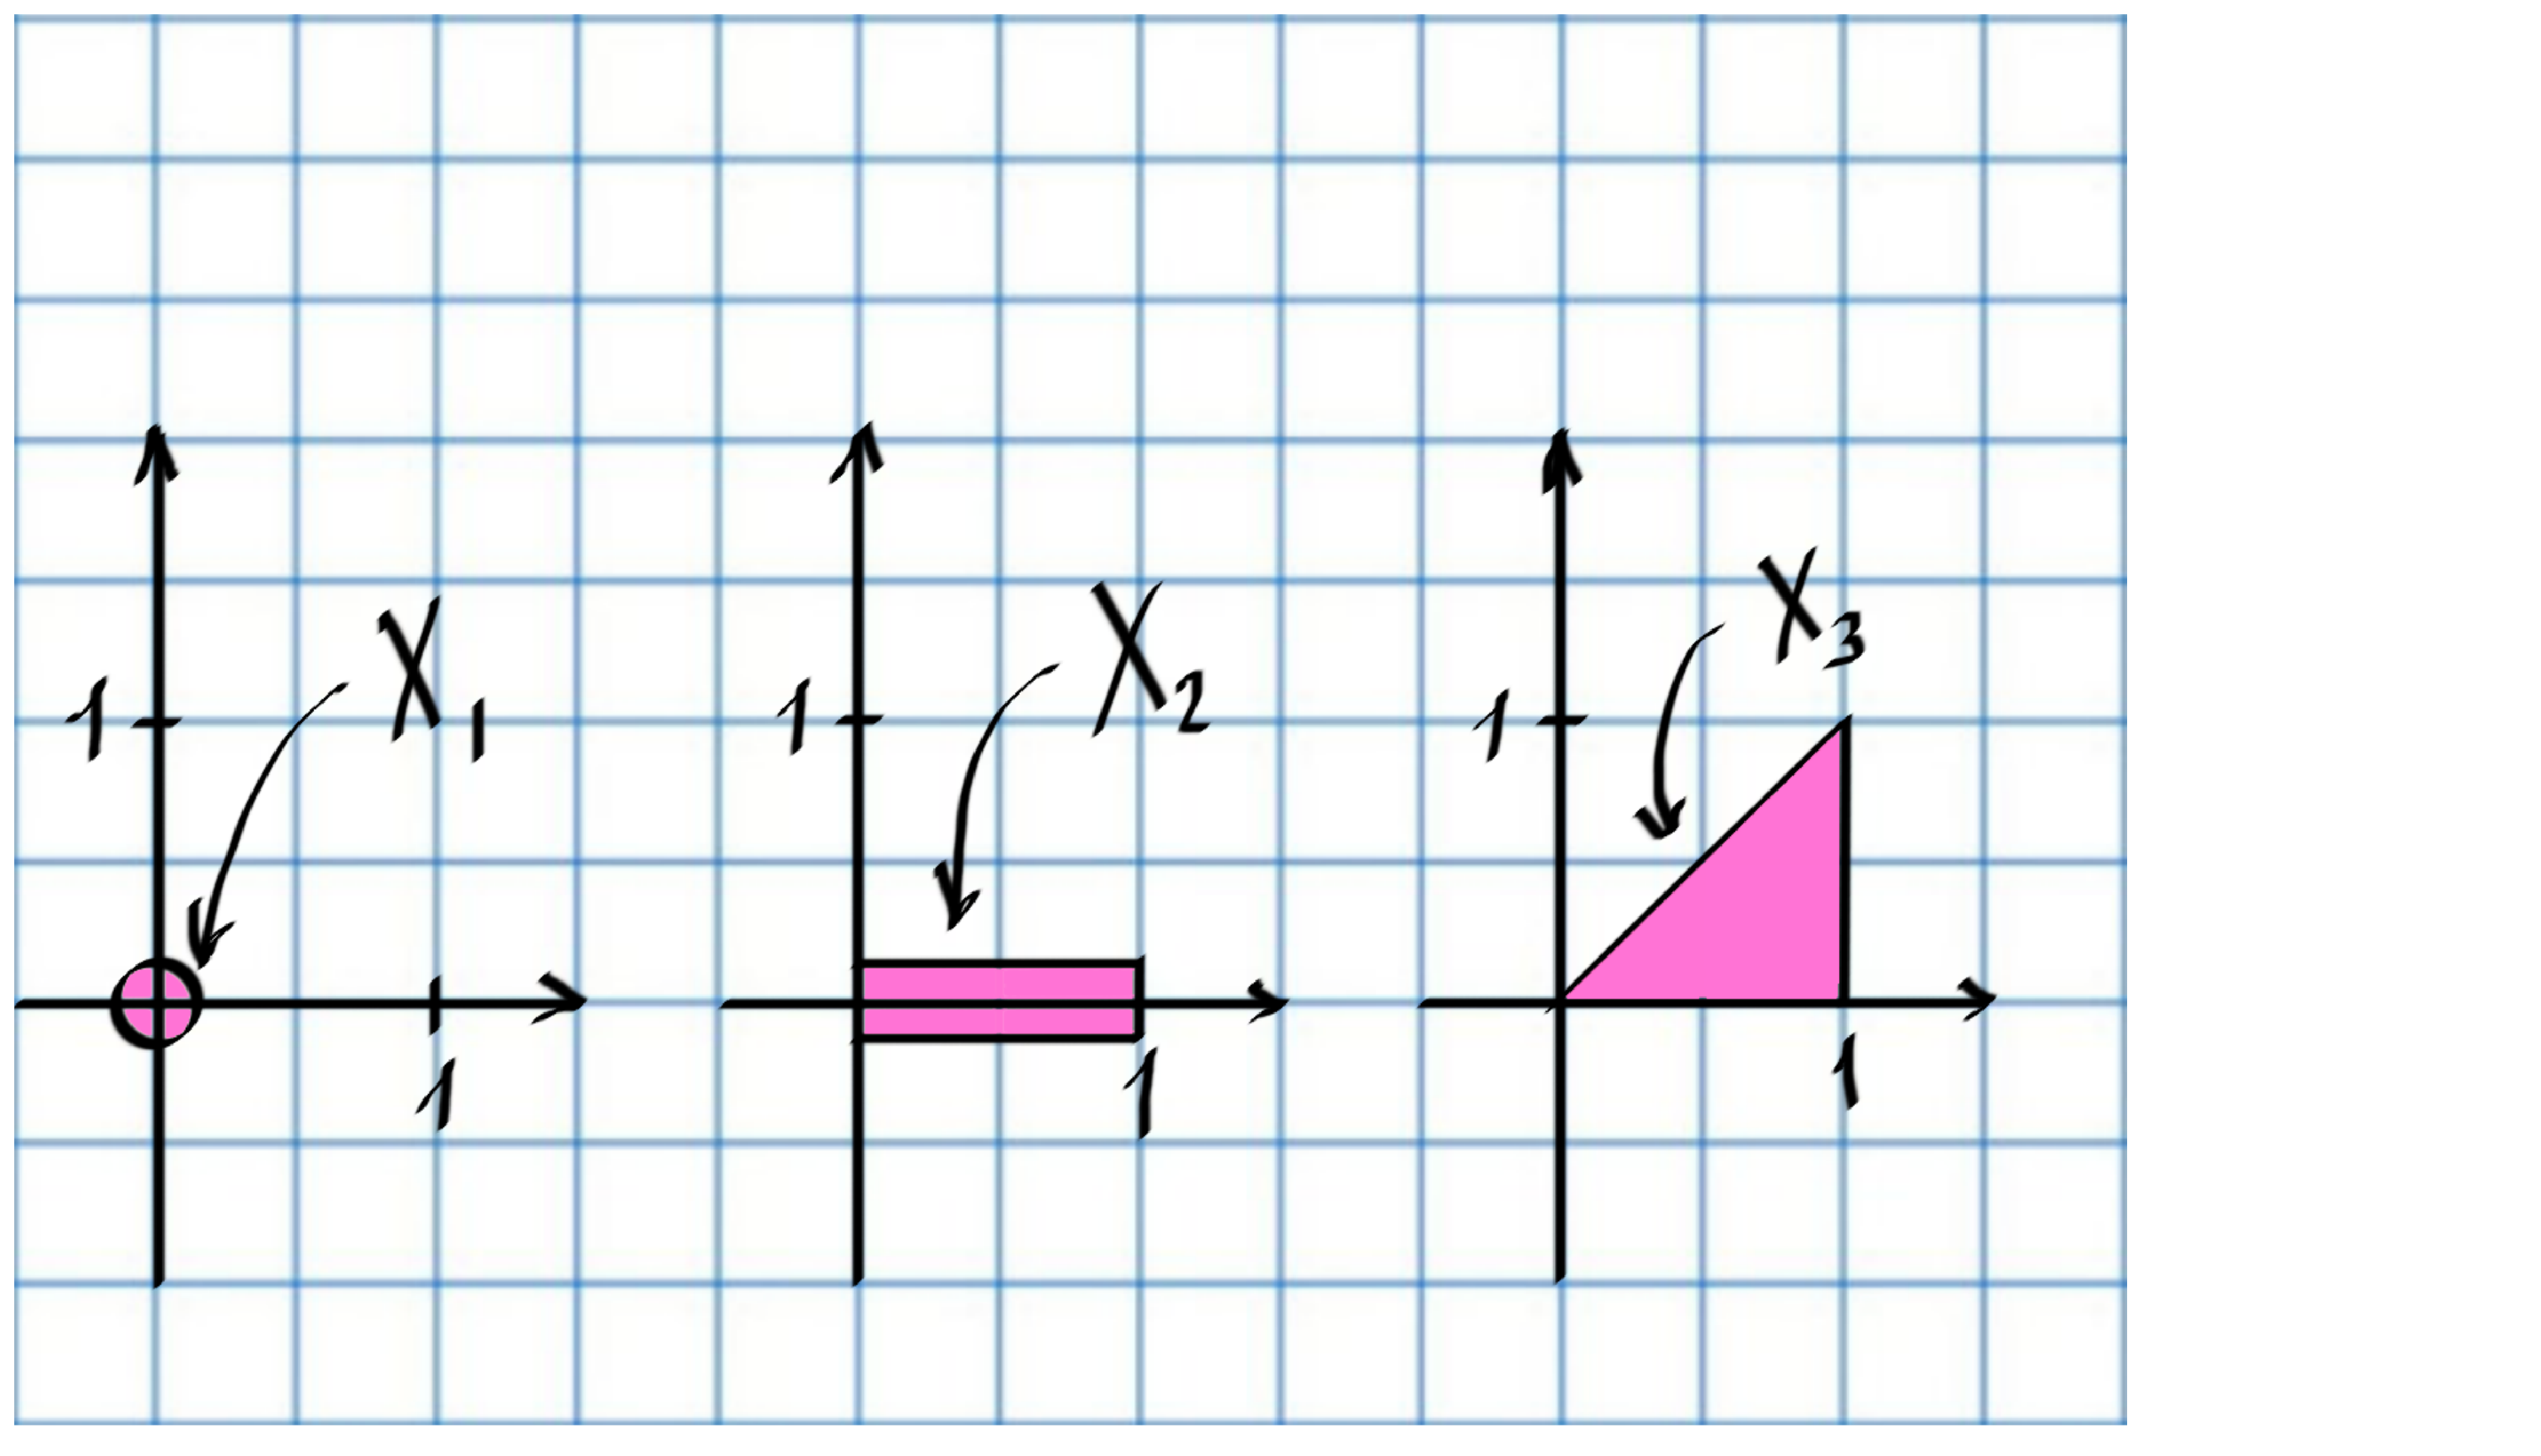
\includegraphics[width=1.2\linewidth]{ris7.eps}
\floatsetup{Рис. 7.}
\end{figure}
\noindent\textcolor[rgb]{0.99,0.05,0.75}{Шаг 2 – изучаем исходные функции.}

Если \textit{f} и \textit{g} – удобные функции, а \textit{c} и \textit{d} – действительные числа, то функция \textit{cf + dg}, которая по определению, принимает на фигуре \textit{F} значение c \textit{f(F)+dg(F)}, очевидно, является удобной.

\begin{spacing}{1.7}
Итак, с удобными функциями можно обращаться как с векторами: их можно умножать на действительные числа и складывать. Положим, например, \textit{P=N}${_2}$\textit{–2N+E} (т. е. \textit{P(F)=N(2F)–2N(F)+1}). Так как функции \textit{N}${_2}$, \textit{N} и \textit{E} – удобные, то и функция \textit{P} – удобная.
\end{spacing}

Сопоставим теперь каждой удобной функции \textit{f}$\in$\textit{Y} вектор в трёхмерном пространстве, а именно, вектор (\textit{f}(\textit{X}${_1}$); \textit{f}(\textit{X}${_2}$); \textit{f}(\textit{X}${_3}$)), где \textit{X}${_1}$, \textit{X}${_2}$, \textit{X}${_3}$ – три целочисленные фигуры, изображенные на рисунке 7. Этот вектор мы будем обозначать через $\stackrel{\rightarrow}{\textit{f}}$. В первых пяти строках таблицы 1 записано, какие векторы сопоставляются уже известным нам удобным функциям.

\noindentТ а б л и ц а  1

\noindent\begin{tabular}{|c|c|c|c|c|}
  \hline
  & \textit{f} & \textit{f}(\textit{X}${_1}$) & \textit{f}(\textit{X}${_2}$) & \textit{f}(\textit{X}${_3}$)      \\ \hline
  1 & \textit{S} & 0 & 0 & 1/2   \\ \hline
  2 & \textit{N} & 1 & 2 & 3   \\ \hline
  3 & \textit{E} & 1 & 1 & 1 \\ \hline
  4 & \textit{N} & 1 & 3 & 6   \\ \hline
  5 & \textit{P} & 0 & 0 & 1   \\ \hline
  6 & \textit{?} & 0 & 2 & 3 \\ \hline
  7 & \textit{e=2E+2S–N} & 1 & 0 & 0   \\ \hline
  8 & \textit{e=N–E–4S} & 0 & 1 & 0   \\ \hline
  9 & \textit{e=2S} & 0 & 0 & 1 \\ \hline
  \hline
\end{tabular}


А всякий ли вектор соответствует какой-нибудь удобной функции (например, вектор (0; 2; 3) из шестой строки)? Положительный ответ на этот вопрос дают строки 7–9 таблицы 1. Из них видно, что удобным функциям e${_1}$, e${_2}$, e${_3}$ соответствуют базисные векторы в трёхмерном пространстве. Поэтому для любых чисел \textit{c}${_1}$, \textit{c}${_2}$, \textit{c}${_3}$ мы можем указать удобную функцию, которой соответствует вектор (\textit{c}${_1}$; \textit{c}${_2}$, \textit{c}${_3}$), а именно – удобную функцию \textit{c}${_1}$\textit{e}${_1}$+\textit{c}${_2}$\textit{e}${_2}$+\textit{c}${_3}$\textit{e}${_3}$. Например, вектор из шестой строки таблицы 1 соответствует функции \textit{2e}${_2}$+\textit{3e}${_3}$=\textit{2}(\textit{N–E–4S})+\textit{3}\cdot\textit{2S=2N–2E–2S}.

\noindent\textcolor[rgb]{0.99,0.05,0.75}{Шаг 3 – критерий совпадения удобных функций.}

До сих пор мы нигде не пользовались тем, что имеем дело с удобными функциями. Любой функции на \textit{Ф} можно было бы сопоставить вектор трехмерного пространства. Например, функции \textit{R} из упражнения 2 соответствует вектор из шестой строки таблицы 1. Особое "удобство" удобных функций заключается в том, что между ними и векторами трехмерного пространства имеется \textit{взаимно однозначное соответствие}. Иными словами, \textit{если f и g удобные функции и если f=g, то функции f и g совпадают}.

Обозначим разность \textit{f–g} через \textit{h}. Тогда утверждение о взаимной однозначности соответствия мужду удобными функциями и векторами принимает такой вид.

О с н о в н а я  т е о р е м а. $\textit{Если}$ \textit{h}$\in$\textit{Y} $\textit{и вектор}$ \stackrel{\rightarrow}{\textit{f}} $\textit{равен нулю, то и функция h есть тождественный нуль}$. 

Мы рекомендуем читателю доказать основную теорему самостоятельно или прочесть доказательство в приложении к статье.

Из основной теоремы сразу следует формула \textit{б)}. Действительно, из первой и пятой строк таблицы 1 мы получаем, что вектор, соответсвующий функции \textit{P–2S} – нулевой. Так как функция \textit{P–2S} удобная, то по основной теореме \textit{P–2S=0}, т. е. \textit{P(F)–2S(F)=0} для любой фигуры \textit{F}. 

\end{multicols}

\end{document}